\documentclass{article}
\usepackage{amsmath}
\usepackage{graphicx}
\usepackage{epstopdf}
\title{CSL603 - Machine Learning\\Lab 2}
\author{Aditya Gupta\\2015CSB1003}
\begin{document}
\maketitle
\section*{Linear Ridge Regression}
Given $X$ and $Y$ we will find $W$ that minimizes $J(W)$, the error function and are defined as:
$$f(X)=
\underbrace{
\begin{pmatrix}
1&x_{11}&\cdots&x_{1D}\\
1&x_{21}&\cdots&x_{2D}\\
\vdots&\vdots&\ddots&\vdots\\
1&x_{N1}&\cdots&x_{ND}
\end{pmatrix}}_{X}
\underbrace{
\begin{pmatrix}
w_0\\w_1\\\vdots\\w_D
\end{pmatrix}}_{W}
=
\underbrace{
\begin{pmatrix}
y_0\\y_1\\\vdots\\y_N
\end{pmatrix}}_{Y}$$
$$
\min_W J(W)\equiv\min_W\frac12(XW-Y)^T(XW-Y)+\lambda||W||^2
$$
Which when solved gives us:
$$W=(X^tX+\lambda I)^{-1}X^TY$$
\subsection*{Observations}
The following observations were obtained:
\begin{itemize}
\item A particular value of $\lambda$(say $0$) was choosen and then the magnitude of entries in the weights $W$ was compared and one by one the least significant ones were discarded and the mean squared error changed in the following way:

\begin{figure}[!h]
\makebox[\textwidth][c]{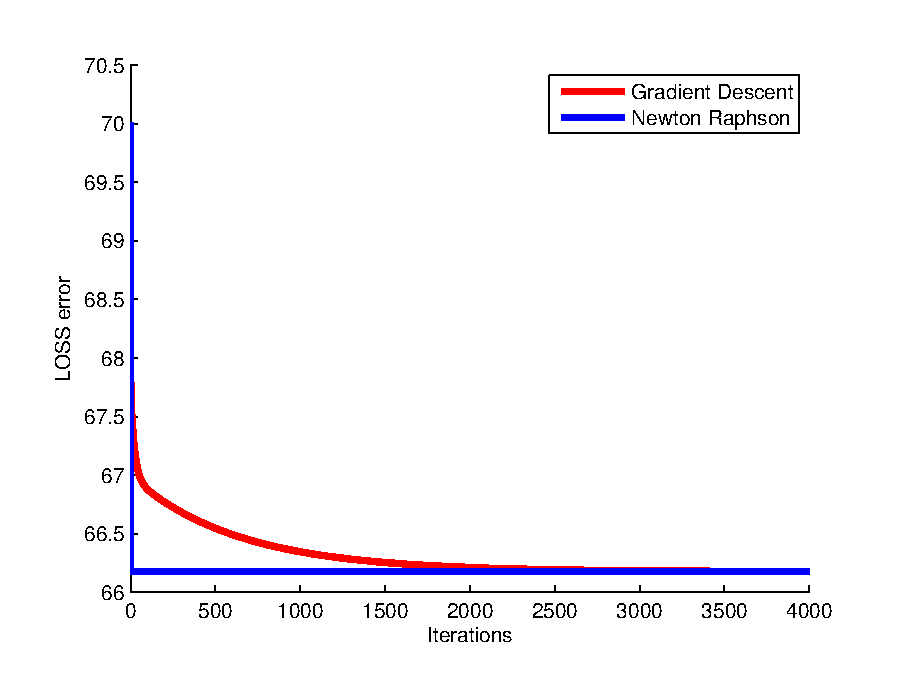
\includegraphics[scale=0.5]{fig1.eps}}
 \caption{Average Mean Sqaured Error for various values of training set fraction and $\lambda$ values used in Ridge Regression for Training Data.}
 \end{figure}
 
 \begin{figure}[!h]
\makebox[\textwidth][c]{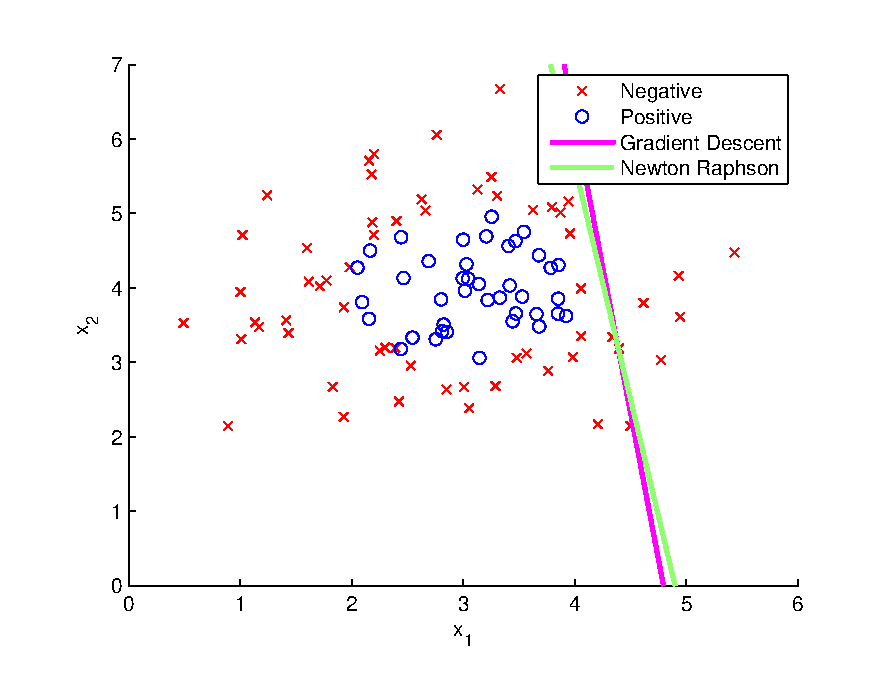
\includegraphics[scale=0.5]{fig2.eps}}
 \caption{Average Mean Sqaured Error for various values of training set fraction and $\lambda$ values used in Ridge Regression for Testing Data.}
 \end{figure}

\item The effect of $\lambda$ on error was observed for different partitions of the data into training and testing sets. The average mean sqaured error for 100 repetitions for splitting-fractions varying from $1\%$ to $99\%$ and lambda values from $0$ to $100$ was observed. The surface corresponding to the average mean absolute error observed was:

\begin{figure}[!h]
\makebox[\textwidth][c]{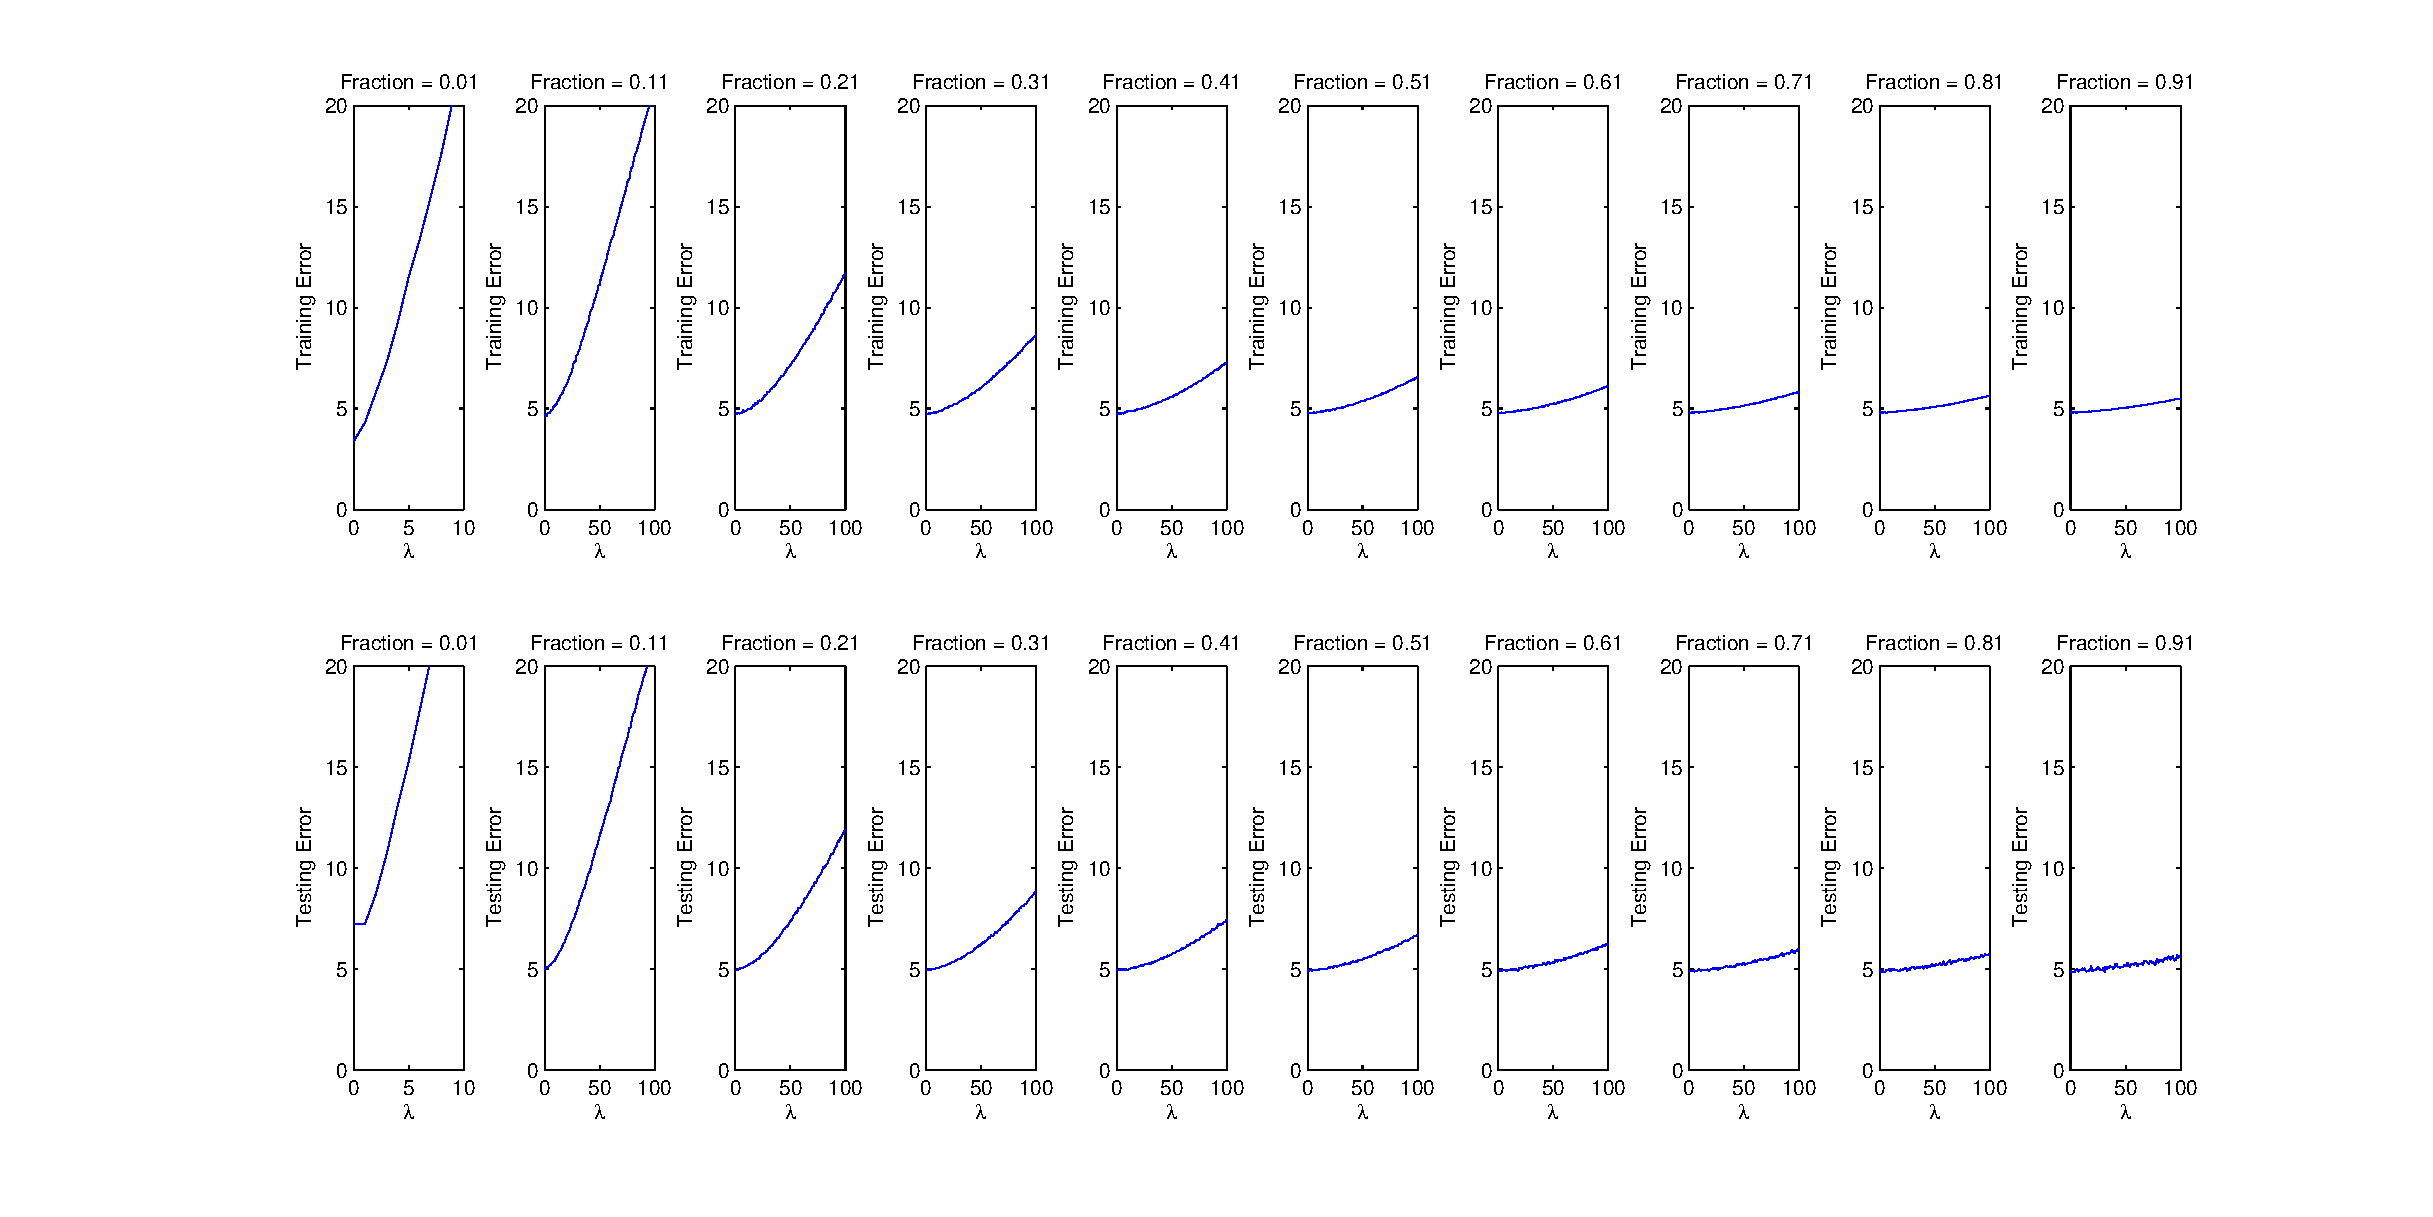
\includegraphics[scale=0.6]{fig3.eps}}
 \caption{Average Mean Squared Error for various training set fractions varying against the $\lambda$ values}
 \end{figure}
 
\item The above surface can be plotted into different graphs for few particular values of splitting-fractions and varying lambda and obsreving the change in average mean absolute error. These figures were observed:



\item Now we noted the minimum average mean squared testing error for each training set fraction values. Also the corresponding $\lambda$ value was observed. These figures were observed:

\begin{figure}[!h]
\makebox[\textwidth][c]{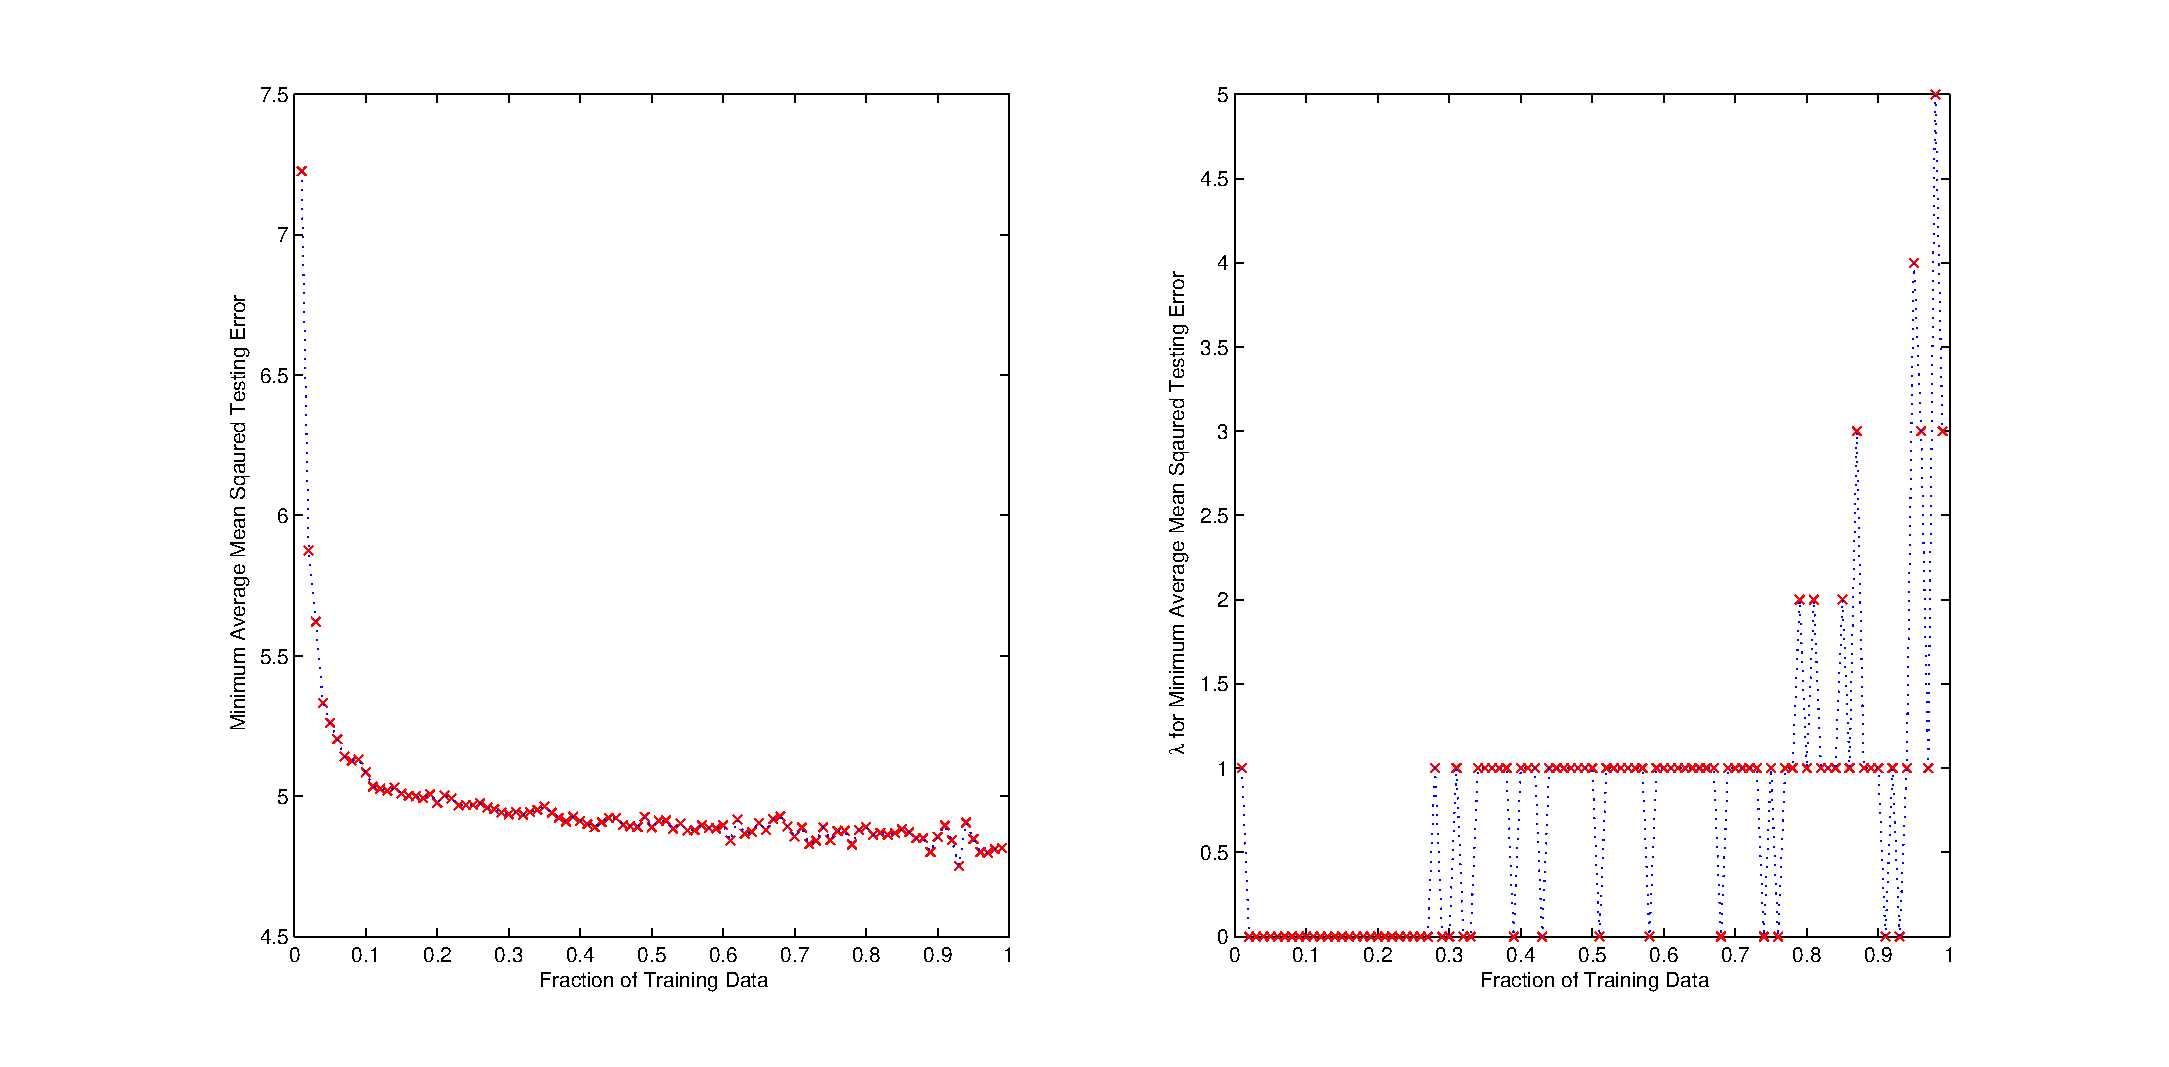
\includegraphics[scale=0.6]{fig4.eps}}
 \caption{Minimum Average Mean Squared Error for various values of training set fraction and the corresponding $\lambda$ values.}
 \end{figure}
 
\item The correspondence between the actual and predicted values was also observed. For perfect prediction, this should correspond to a straight line through origin at $45^\circ$ degrees. The following figures were obtained:

\begin{figure}[!h]
\makebox[\textwidth][c]{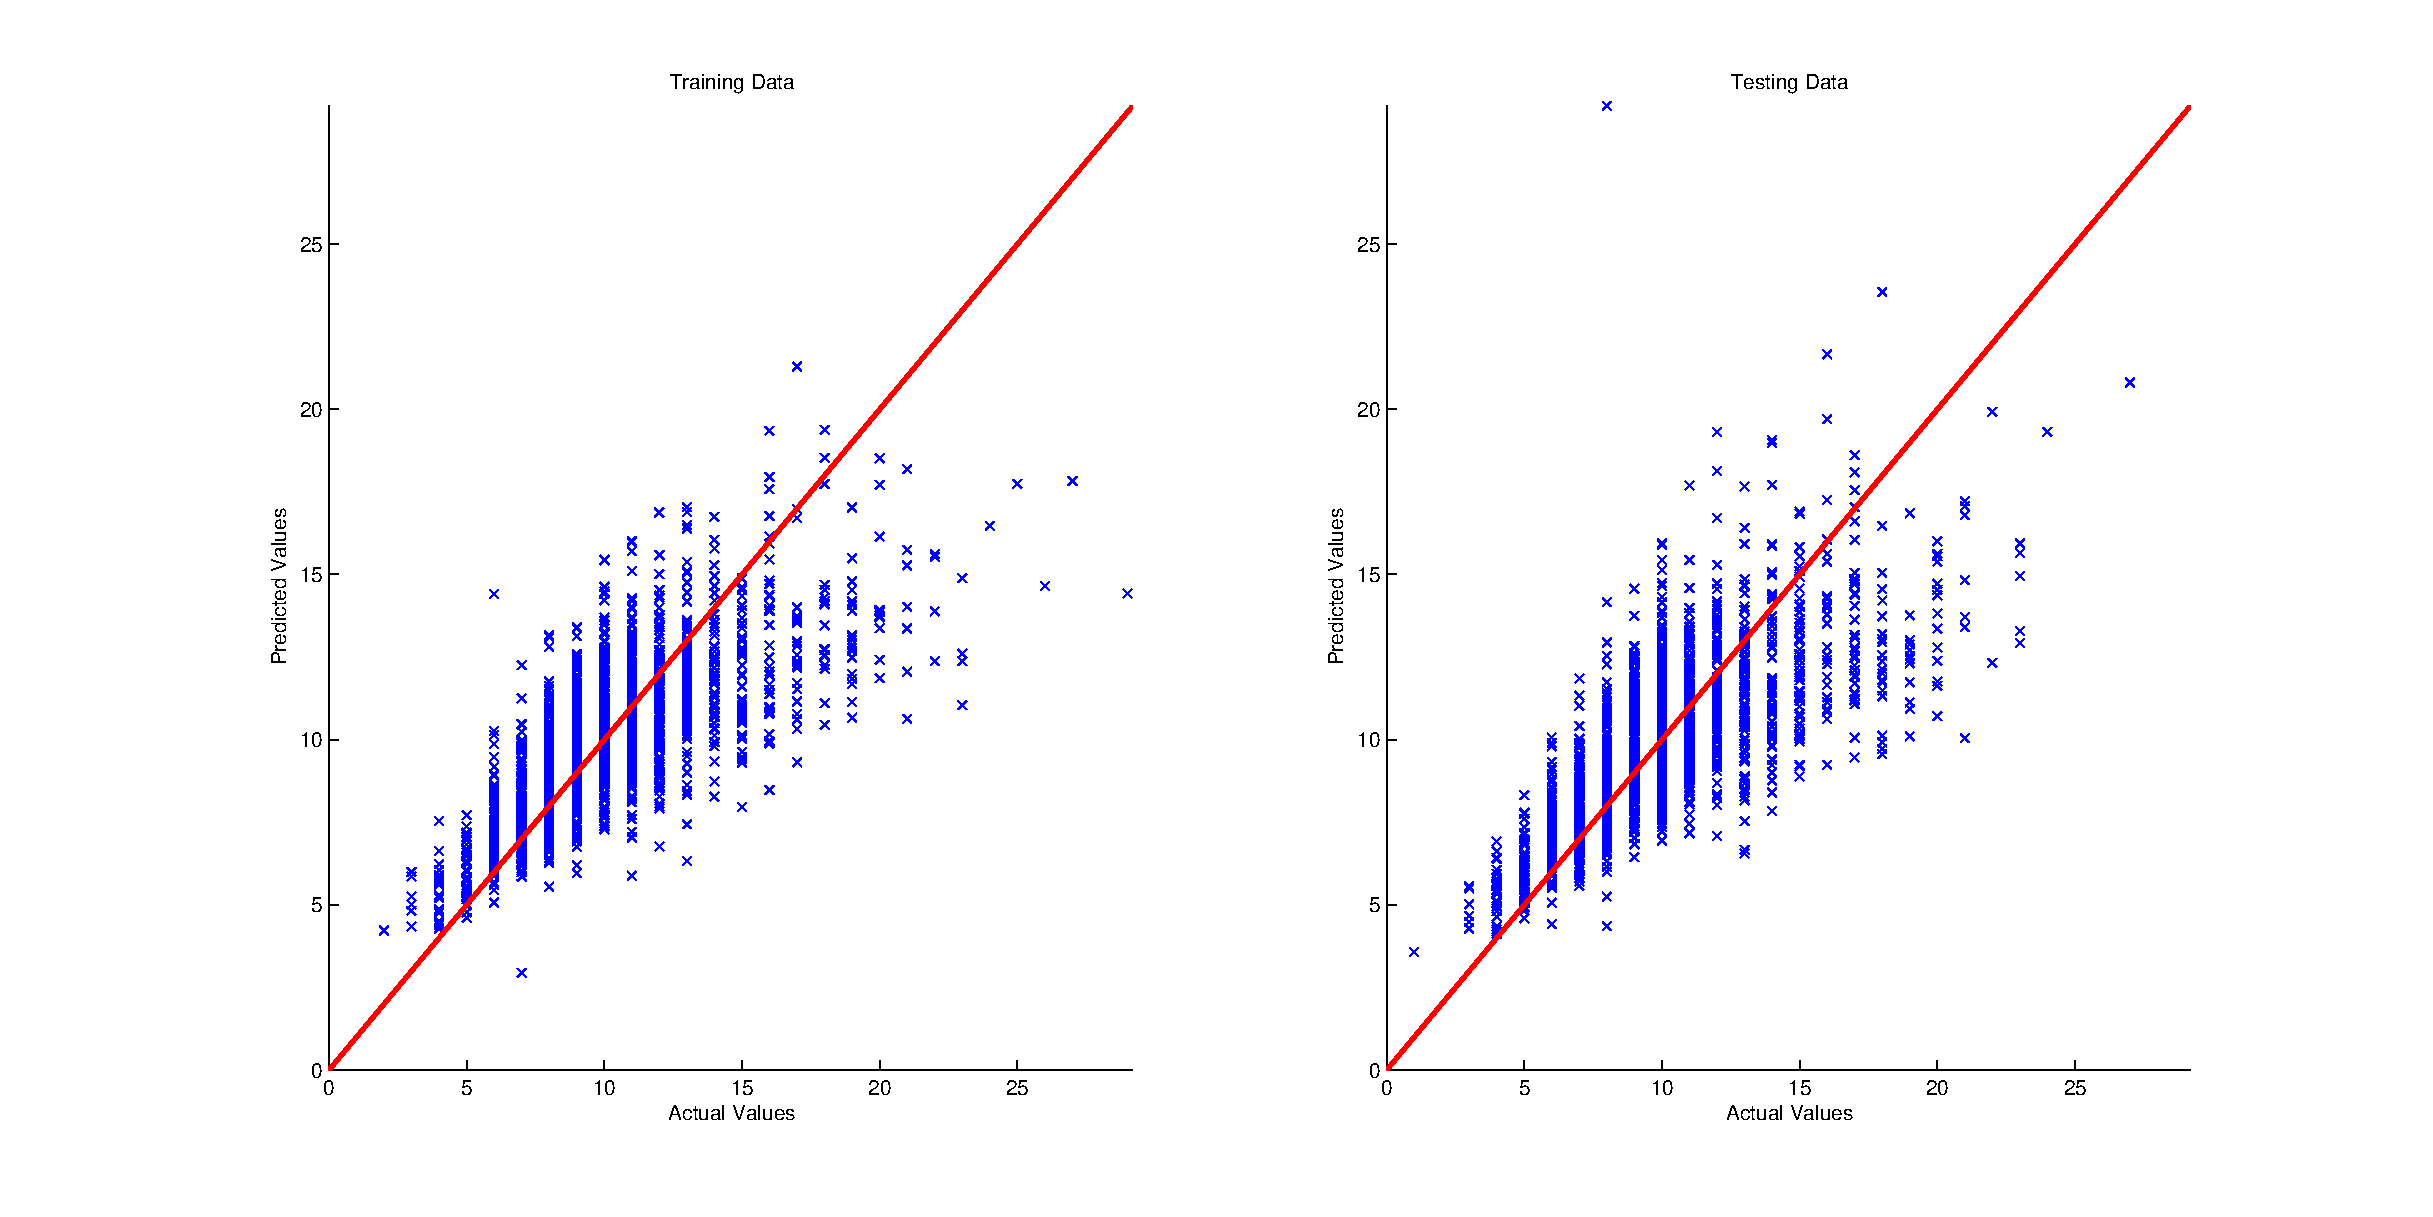
\includegraphics[scale=0.6]{fig5.eps}}
 \caption{Relation between the actual data set values and predicted values for training and testing data. The reference line $y=x$ is shown in red.}
 \end{figure}
 
\end{itemize}
\end{document}